\section{Data and Accounting Boundaries}
\label{sec:data}

Pakistan Civil Aviation Authority (PCAA) statistics provide the activity controls. The
FY2023--24 airport report records 40,600 domestic and 95,267 international commercial
movements, 21,223 non-commercial movements and 5.680 million domestic passengers
\citep{pcaaairports2024}. A separate airline report gives departures, arrivals, passengers,
cargo and mail by operator \citep{pcaaairlines2024}. One movement is one take-off or landing;
the national domestic activity control is therefore 20,300 flight stages. The historical
movement series covers FY2006--07 to FY2023--24.

OCAC sectoral reports provide the fuel control. In FY2023--24 they record
\SI{193813}{\tonne} of JP-1 for ``Domestic Avi--PIA'', \SI{166119}{\tonne} for ``Domestic
Avi--Others'' and \SI{283147}{\tonne} for ``Overseas/Foreign Aviation'', with government
JP-1, JP-8 and 100LL retained separately \citep{ocacaviation}. Final reports supply nine annual
fuel accounts from FY2016--17 to FY2024--25; public cumulative reports supply 42 months that
overlap OECD completely. Revisions and category-label changes are versioned rather than
silently harmonised \citep{ocacarchive}.

OECD monthly aviation estimates cover calendar 2019--2024 and distinguish domestic and
international territory emissions from resident- and non-resident-carrier activity
\citep{oecdaviation}. In FY2023--24 they report 235.8 kt \COtwo{} for domestic territory
aviation and 1812.0 kt for international aviation. Resident carriers account for 227.0 kt of
domestic and 657.3 kt of international-departure emissions. Their domestic share supplies the
central fuel partition; OECD remains an external comparison for models that do not use that
share.

Pakistan's Biennial Transparency Report, Third National Communication and 2026 Common
Reporting Table (CRT) package provide the official national comparison
\citep{pakbtr2024,paknc32025,pakcrt2026}. The CRT workbook supplies calendar-2022 emissions,
energy activity, fuel notation and an explicit domestic/international distribution. Climate
TRACE v7 supplies national monthly and airport-source records for an exact FY2023--24 temporal
and spatial comparison \citep{climatetrace}. ICAO route factors, OpenAP, public ADSB.lol traces
and ERA5 meteorology support the model-resolution and sensitivity analyses; their detailed
adapters and coverage limits are documented in the supplement
\citep{sun2020openap,adsblolhistory,era5arco}.

Table~\ref{tab:source-roles} fixes each source's evidentiary role before results are examined.
In particular, ``external'' does not automatically mean independent, and a calibration input
is never counted as validation.

\begin{table*}[htbp]
\centering
\footnotesize
\begin{tabular}{@{}p{0.18\linewidth}p{0.31\linewidth}p{0.25\linewidth}p{0.13\linewidth}@{}}
\toprule
\textbf{Source/comparison} & \textbf{Role} & \textbf{Shared input or boundary constraint} & \textbf{Evidence class} \\
\midrule
PCAA airport and airline reports & Movement, passenger and margin controls & One reporting system for activity and load checks & Targeted control \\
OCAC total vs OECD combined & Gross fuel--flight closure & Carbon conversion only & Largely independent \\
OCAC bridge vs OECD domestic & Resident-customer partition & OECD share used directly & Calibration \\
Movement/route models vs OECD & Domestic territory comparison & Possible generic ICAO conventions & External, partial \\
Pakistan CRT vs OECD & Official-boundary diagnostic & Inventory year only & External, largely independent \\
PCAA airports vs Climate TRACE & Spatial ordering & Possible surveillance/performance overlap & Corroboration \\
ADSB.lol and ERA5 & Coverage and weather sensitivities & Reconstructed routes or airport coordinates & Supplementary diagnostics \\
\bottomrule
\end{tabular}
\caption{Data roles and comparison independence. The evaluation does not promote any source
to a universal truth benchmark.}
\label{tab:source-roles}
\end{table*}

\begin{figure*}[htbp]
\centering
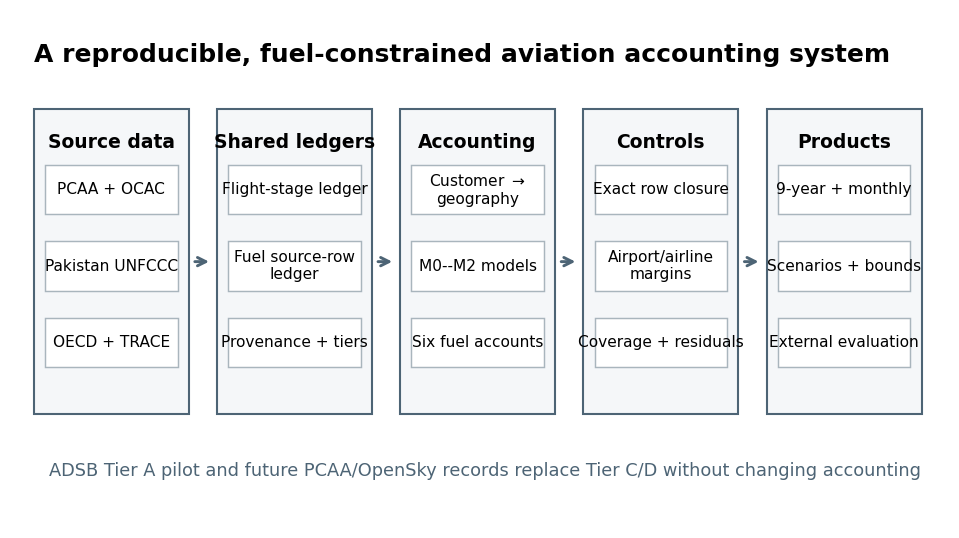
\includegraphics[width=0.94\textwidth]{aviation_framework.png}
\caption{Data sources populate conserved fuel and flight ledgers, from which accounting
products, domestic model estimates and external evaluations are generated.}
\label{fig:framework}
\end{figure*}
